% Evaluation

\chapter{Results and Evaluation} % Main chapter title

\label{Chapter6} % For referencing the chapter elsewhere, use \ref{Chapter4} 

\lhead{Chapter 6. \emph{Results \& Evaluation}} % This is for the header on each page - perhaps a shortened title

%----------------------------------------------------------------------------------------

Success of any project or product depends on many factors - the performance, design, innovation and design. Each of the elements it consists of contribute to at least one of them. 
In this chapter we evaluate our project in attempt to assess its success.

First, we focus on quantitative analysis. We present the results of testing and validating of our neural network for music emotion prediction using fresh and unseen data and contrast them with existing literature. Then we move on to evaluation of the boundary detection system by comparing the performance and accuracy it yields with two other algorithms. Finally, we examine the results of the labelling algorithm.

Last, but not least, we move on to user experience research. We go over user testing and its outcome, as well as how it was used to further improve our game. 

\vspace{10pt}

\section{Evaluation of Mood Detection system}

\begin{figure}[t]
    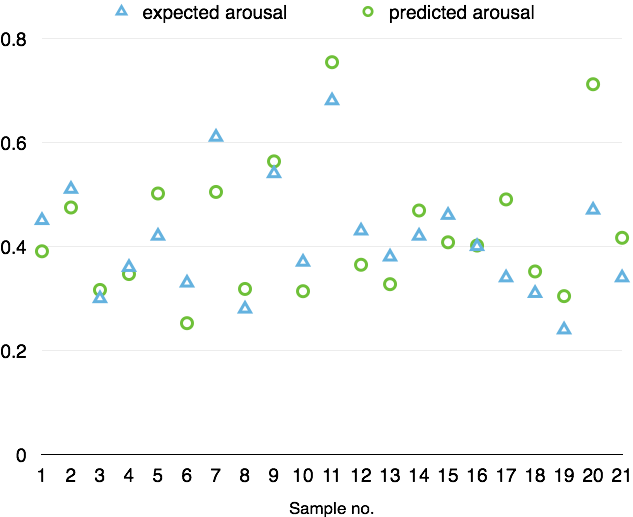
\includegraphics[width=0.7\textwidth]{Figures/finalarousal}
    \centering

  \caption{A plot of the expected and predicted .}
  \label{fig:anneval}
\end{figure}


We designed our neural networks to as means of calculating valence and arousal ratings of songs using audio features we extract. 

To evaluate its performance we have to have a way of telling how successful it is in guessing the values. To achieve this, we activated the network on 21 unseen music tracks that we knew valence and arousal values of and gathered the output network produced for it. Then, we computed the root mean square error between the ground truth ratings and network-predicted outputs across all segments of all the test melodies. The network's performance total RMSE was 0.08895 on scale from 0 to 1 or 9\%. The plot of the expected and predicted values can be seen in Figure \ref{fig:anneval}.

In contrast, in their paper \cite{vempala} Vempala and Russo trained a neural network with 1.14 error on scale 1 to 9, or 14.3\%.

If we look at the two predicted values separately, the coefficient of determination for the arousal reached 59.24\% and 40.34\% for valence.

In comparison, Yang and Lin \cite{mood} achieved a lower success rate, as their $R^2$ scored 58.3\% for arousal and 28.1\% for valence. 


\begin{figure}[t]
    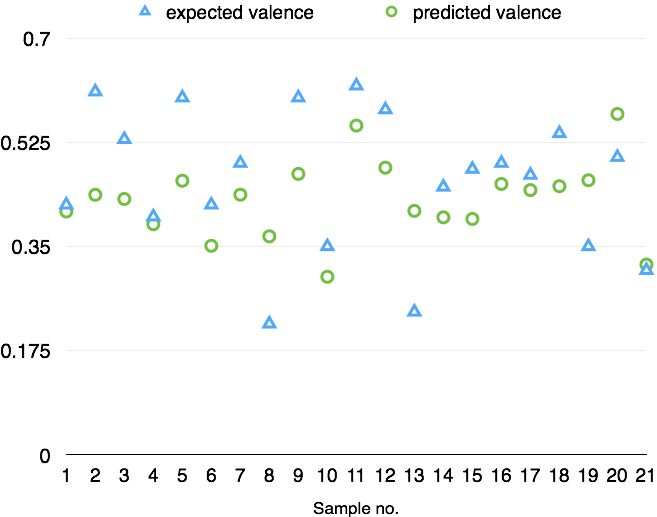
\includegraphics[width=0.7\textwidth]{Figures/finalvalence}
    \centering

  \caption{A plot of the expected and predicted valence.}
  \label{fig:anneval}
\end{figure}


Results from the static network indicate that a network can be trained to identify statistical consistencies across audio features abstracted from music and satisfactorily predict valence/arousal values that closely match mean participant ratings.


\begin{table}
\begin{center}
\begin{tabular}{| c | c | c | c | } \hline 
 expected arousal & expected valence & predicted arousal & predicted valence \\ \hline \hline

0.45  & 	0.42  &  0.390444 &  0.408524   \\ \hline
0.51	&  0.61  &  0.474538 & 0.436625   \\ \hline
0.3    &  0.53  &  0.316230 & 0.429643   \\ \hline
0.36	&  0.4    &  0.346713 & 0.387249   \\ \hline
0.42	&  0.6    &  0.501414 & 0.460295   \\ \hline
0.33	&  0.42  &  0.252398 & 0.350910  \\ \hline
0.61	&  0.49  &  0.504392 & 0.436785   \\ \hline
0.28	&  0.22  &  0.318096 & 0.366836   \\ \hline
0.54	&  0.6    &  0.563120 & 0.471717   \\ \hline
0.37	&  0.35  &  0.313782 & 0.298909   \\ \hline
0.68  &  0.62  &  0.753534 & 0.552922   \\ \hline
0.43	&  0.58  &  0.364568 & 0.482194   \\ \hline
0.38	&  0.24  &  0.327288 & 0.409628   \\ \hline
0.42  &  0.45  &  0.468762 & 0.398749   \\ \hline
0.46  &  0.48  &  0.407701 & 0.396029   \\ \hline
0.4    &  0.49  &  0.401469 & 0.454892   \\ \hline
0.34  &  0.47  &  0.490065 & 0.444592   \\ \hline
0.31  &  0.54  &  0.351714 & 0.451086   \\ \hline
0.24  &  0.35  &  0.304314 & 0.461078   \\ \hline
0.47	&  0.5    &  0.711224 & 0.572459   \\ \hline
0.34	&  0.31  &  0.416320 & 0.319491   \\ \hline
\end{tabular}
\caption{Table showing the root mean square error for training the network for given number of nodes in the hidden layer.}
\label{table:rsmetablefinal}
\end{center}
\end{table}



\section{Boundary Detection}

The first towards the evaluation of the segmentation algorithm was to gather the ground truth data to test against. To remove bias caused by personal preferences in music, we sought external sources for help in selection of the tracks. This is why we consulted the top charts created by music magazines and online portals such as Rolling Stone, Billboard, Gibson etc. The full list can be found in \cite{toplists}.

Once we have retrieved the lists with the most popular songs across genres, we selected one song per top list based on our familiarity. Although this might introduced some sort of personal preference into the dataset, it also allowed us to more intuitively create the ground truth data, as the familiarity with a song makes the manual labelling more obvious. For instance, in “Blitzkrieg Bop” by The Ramones, the bridge is repeates as often as verse and chorus, which is bound to introduce confusion to a person who hears the song for the first time and is asked to segment and label it.

In totall, we manually labelled 10 songs:
\vspace{-10pt}
\begin{description}
\itemsep0em 
\item[“The Number of The Beast”] by Iron Maiden (Metal)
\item[“Rock With You”] by Michael Jackson (Soul/R\& B)
\item[“Blitzkrieg Bop”] by The Ramones (Punk Rock)
\item[“This Land is Your Land“] by Woody Guthrie (Folk)
\item[“One More Time”] by Daft Punk (Dance)
\item[“Smooth”] by Santana (featuring Rob Thomas) (Pop)
\item[ “Crazy in Love”] by Beyonce (featuring Jay-Z) (Pop / Rap)
\item["Help!"] by The Beatles (Rock)
\item["Respect"] by Aretha Franklin (R\& B)
\item["Back in the USSR"] by The Beatles (Rock)
\end{description}

For each of the songs, we conducted 5 measurements to manually detect the boundaries. Once we have gathered the data, we averages each bound to create ground truth with reference boundaries and labels.

To be able to fully evaluate the performance of our algorithm in comparison with state-of-the-art solutions already existing, we also gathered data produced by two other algorithms. The first one, described by Foote and Cooper \cite{FooteCooper}, is a classic approach applying a "“checkerboard” kernel over the diagonal of a self similarity-matrix (SSM). The other one is an approach published by Kaiser and Sikora \cite{Sikora}, with use of non-negative matrix factorisation on only one feature. 

We conducted two types of studies to determine the performance of our bound finding algorithm.

First and the most intuitive one is the comparison of amount of boundaries detected. If an algorithm returns a smaller amount of segments it means that most probably its detection system is not sensitive enough - it merges some of bounds into bigger ones. And vice versa - if the algorithm returns more boundaries than the ground truth, it means it picked on song segments that differ in a less obvious way and, hence, its output is too granular.


\begin{table}
\begin{center}
\begin{tabular}{| c | c | c | c | c | } \hline 
Song  								& Ground	& Foote 	&  Kaiser 	& Ours \\ \hline \hline
The Number of The Beast 	&	17			& 	9  			&  15 		&  20   	\\ \hline
Rock With You					&	11			&  9			&  15 		& 17   	\\ \hline
Blitzkrieg Bop 					&	14			&  9  			&  14 		& 14   	\\ \hline
This Land Is Your Land 		&	11			&  9			&  12 		& 7    	\\ \hline
One More Time					&	13			&  9    		&  14 		& 17   	\\ \hline
Smooth								&	14			&  9  			&  14 		& 16  	\\ \hline
Crazy In Love					&	17			&  9  			&  13  		& 16   	\\ \hline
Help!									&	10			&  9		   	&  17 		& 12   	\\ \hline
Respect								&	12			&  9  			&  14 		& 12  	\\ \hline
Back In the USSR				&	15			&  9  			&  13		    	& 14		\\ \hline \hline
RMSE								&	N/A		& 4.98		&  3.08		& 2.95	\\ \hline 

\end{tabular}
\caption{Table showing the root mean square error for training the network for given number of nodes in the hidden layer for the checkerboard algorithm (by Foote, \cite{FooteCooper}), NMF based algorithm (by Kaiser, \cite{Sikora}) and ours.}
\label{table:evalStructureCount}
\end{center}
\end{table}


The results of our investigation can be seen in Table \ref{table:evalStructureCount}. By calculating the root mean square error for outputs of every algorithm, we noticed that our algorithm has a slightly better performance than the simple non-negative matrix factorisation one. On the other hand, checkerboard designed by Foote and Cooper consistently returned 9 labels, and hence yielding the worst performance.

Apart from observing the RMSE of the boundary number, we reasoned about the distribution of the results. In particular, we believe that the situation when the algorithm is over-segmenting, returning more bounds than there are in the ground truth, is better than the one when the structure retrieval system is not sensitive enough and merges boundaries that do not belong together. This is especially true in case of our application, where if more boundaries are returned, the mood detection becomes more accurate at expense of efficiency. On the other hand, with every lost bound we lose precision in the mood detection in two neighbouring segments.

If we look at Figure \ref{fig:boundcount}, we can see that in the light of our previous observations, the checkerboard yields a dramatically worse performance than nmf and our algorithm. In contrast, the latter two exhibit the same proportion of over- and under-segmenting.


\begin{table}
\begin{center}
\begin{tabular}{| c | c | c | c | c | } \hline 
Song  								& 	500ms 			&  3s						&  deviation	\\ \hline \hline
The Number of The Beast 	&	Foote			& 	Foote  				&  Ours 			\\ \hline
Rock With You					&	Ours				&  Ours			  		&  Ours			\\ \hline
Blitzkrieg Bop 					&	Kaiser			&  Ours  				&  Ours 			\\ \hline
This Land Is Your Land 		&	Ours				&  Foote			  	&  Foote 		\\ \hline
One More Time					&	Foote			&  Foote    				&  Ours 			\\ \hline
Smooth								&	Foote			&  Foote  				&  Ours 			\\ \hline
Crazy In Love					&	Ours				&  Ours  				&  Ours  		\\ \hline
Help!									&	Ours				&  Foote		   		&  Ours 			\\ \hline
Respect								&	Foote			&  Ours  				&  Ours 			\\ \hline
Back In the USSR				&	Ours/Kaiser	&  Ours/Kaiser 		&  Ours		    	\\ \hline

\end{tabular}
\caption{Table showing the best performing algorithm in each category for all the songs.}
\label{table:evalStructureRank}
\end{center}
\end{table}


\begin{wrapfigure}{r}{0.5\textwidth}
\vspace{-10pt}
  \begin{center}
    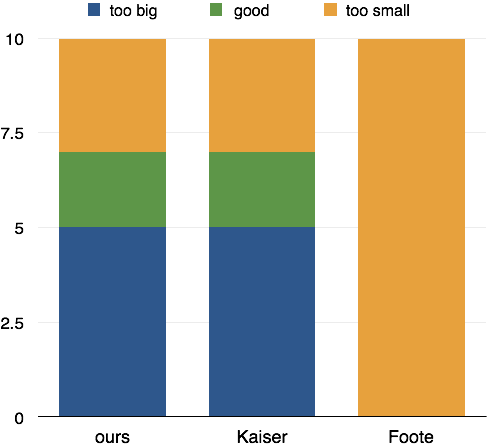
\includegraphics[width=0.48\textwidth]{Figures/count}
  \end{center}
  \caption{Figure presenting the amount of each type of errors produced by all the evaluated algorithms.}
\label{fig:boundcount}
\end{wrapfigure}

Another measurement of success of our boundary retrieval is computation of boundary detection hit-rate. A hit is counted whenever a reference boundary is within a certain window of an estimated boundary. An important thing to note is that each boundary should be matched at most once, otherwise we can get some irrelevant results. For instance, if we are estimating the algorithm with window size 3 seconds, in the ground truth there are two boundaries 6 seconds apart and our algorithm detects only one right in the middle, if we do not exclude the boundary once compared with the first one in the ground truth, the performance of our algorithm will be ranked as much better than it actually was. 


In addition to computing the hit-rate for windows of sizes 500ms and 3s, we also computed the median deviations between the reference and estimated boundaries of the song. In particular, we focused on median time from each reference boundary to the closest estimated boundary.

We implemented our evaluation benchmark using Python mir\textunderscore eval library \cite{mireval}.
Again, to best evaluate performance of our algorithm, we compare the results it yields with results of the checkerboard and NFM based ones. Our findings can be seen in Table \ref{table:evalStructureRank}.


\begin{wrapfigure}{r}{0.5\textwidth}
\vspace{-30pt}
  \begin{center}
    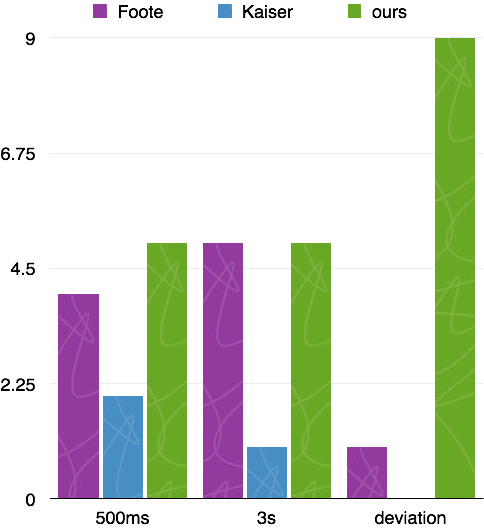
\includegraphics[width=0.48\textwidth]{Figures/structurechamps}
  \end{center}
  \caption{Chart presenting amount of times every algorithm excelled in each of the categories - hit-rate with window sizes of 500ms and 3s and the median deviation from the ground truth.}
\label{fig:structurechamps}
\end{wrapfigure}

As we can see in the Figure \ref{fig:structurechamps}, in the majority of cases, the performance of the algorithm designed by Kaiser falls behind the other two methods. It ranked as first twice when calculating the hit-rate with the window size w=500ms, once for the w=3s and it never excelled in the deviation category. On the other hand, the algorithm designed by Foote and Cooper yields similar overall performance as ours when evaluating hit-rate with w=3 and slightly worse for 500ms. This most probably is caused by the fact that in many cases our algorithm managed to find the segments but was a bit off, not qualifying for the 500s window. However, once the window got increased, its performance improved more than in case of the ``checkerboard'' algorithm. The exact results can be seen in section \ref{sec:segevalapp} in Appendix C. 

In conclusion, we believe that the algorithm for boundary detection we created is suitable for our application and yields performance comparable or exceeding the state-of-the-art creations in its field. 

\section{Labelling}


\section{Questionnaires}
Questionnaires are one of the most common and popular tools to gather data from a large number of people. They generally consist of a limited number of questions that ask participants to rate the effectiveness of various aspects of the activity. The questions should focus on the key points we are trying to evaluate. 

Questionnaires tend to be short in order to reduce the amount of time respondents need to complete them, and therefore increase the response rate. 

We composed questionnaires that are quantitative and generally consist of close-ended questions (tick the box, or scales), as the open ended questions tent to make data analysis and reporting more difficult.

\subsection*{Preliminary Research}

Before the design and implementation phase of the project, we conducted a study to determine what features could be desirable in the game. We led a survey among 18 people aged 17-25 asking about their past experience with music rhythm games. 
The questions and the results are presented in the Table \ref{table:preliminaryquestions}. Each of the questions was answered on a scale from 1 to 5, where 1 is a No,  3 is Neutral and 5 is a Yes.

\begin{table}
\begin{center}
\begin{tabular}{| p{8cm} | c | c | c | c | } 																								      \hline 
\textbf{Question} & \textbf{Average} & \textbf{Stdev} & \textbf{Min} & \textbf{Max} 						   \\ \hline \hline
Do you like playing games? & 4.11 & 0.9 & 2 & 5		 					 					 									\\ \hline 
Do you like listening to music? & 4.67 & 0.59 & 3 & 5		 					 					 								\\ \hline 
Do you often play games? & 3.722 & 0.89 & 2 & 5 		 					 					 								\\ \hline 
Have you ever played Guitar Hero or other rhythm music game? & 3.88 & 1.84  & 1 & 5							\\ \hline 
Did you feel like the choice of songs was limiting you? & 3.22 & 1 & 1 & 5 					 							\\ \hline 
Were you able to load in your song of choice in there? & 2. & 1.41 & 1 & 5 					 							\\ \hline 
Would you like to be able to load a song into it? & 4.27 & 0.82 & 3 & 5 				 									\\ \hline 
Did you feel like the game graphics were reflecting the emotions in the song? & 2.78 & 1.06 & 1 & 4 			\\ \hline 
Would you like the game to reflect the emotions in the song? & 3.67 & 0.84 & 3 & 5 	 								\\ \hline 
Was the game reflecting the section of the song you were in? & 2.44 & 1.25 & 1 & 4  								\\ \hline 
Do you feel it would be useful to know what section of the song is currently played? & 3.5 & 0.86 & 2 & 5  	\\ \hline 
\end{tabular}
\caption{Table presenting the results of the preliminary questionnaire.}
\label{table:preliminaryquestions}
\end{center}
\end{table}

As we can see from the Table \ref{table:preliminaryquestions}, the majority of young people surveyed did enjoy playing games to a similar extent. However, the results of the survey tell us that listening to music is almost unanimously beloved activity, with the highest average result and the smallest standard deviation. 
Majority of people play games quite often, but the lower average and standard deviation compared to the first question suggests that there are some people who enjoy playing games a lot but they do not spend that much time doing so, be it due to lack of time or other arrangements. 

When it comes to rhythm-games specific questions, most people have played a game of such type before. A majority of people believed that having a set playlist was limiting their experience, however, there were some who did not mind this that much. However, when asked if the ability to upload their own music would improve their experience, everybody was either neutral of agreed - nobody was against the idea. 

Majority, but no all surveyed believed that the rhythm game they played did not reflect the mood of the song they played, which can be deducted from the average below the neutral value 3 with the maximum value being four, so above the neutral. They believed it would be nice for the game to reflect the emotions in the song, but the need expressed was not as urgent as in case of the upload of their own songs. On the other hand, nobody opposed to such feature, which is reflected by the minimum value given being three.

Finally, we asked the surveyed whether they felt like the game was reflecting the built of the song, notifying them of where in the song they were. Most agreed that the games like that did not contain any sort of visualisation for the song segmentation. Majority of surveyed agreed that such feature would be useful, although a small amount of people believed it would not contribute in any way, answering with 2.

We also had to additional questions asking for suggestions, in case there are other features that could be useful to the game or could make the game more attractive that we missed in our initial market research. 

\subsection*{Final Research}

For our final research, we demonstrated our game to a group of 8 people aged 18-23 and asked them to fill in a questionnaire to describe their experience and thoughts on the game. Each of the questions was answered on a scale from 1 to 5, where 1 is a No,  3 is Neutral and 5 is a Yes. The questions and the results are presented in the Tables \ref{table:finalquestionsinterface}, .

\begin{table}
\begin{center}
\begin{tabular}{| p{8cm} | c | c | c | c | } 																	  \hline 
 \textbf{Question} & \textbf{Average} & \textbf{Stdev} & \textbf{Min} & \textbf{Max } \\ \hline \hline
 I knew what to do in the game straight away. 				& 4.88 & 0.35 & 4 & 5		   \\ \hline 
 I needed hints to play the game. 								& 2.25 & 1.58 & 1 & 5 	   \\ \hline 
 I needed somebody to tell me how to play the game. 	& 1.13 & 0.35 & 1 & 2  	   \\ \hline 
 I liked the design of the menu. 									& 3.86 & 0.99 & 2 & 5   	   \\ \hline 
 I felt like the game interface was too crowded. 				& 1.38 & 0.51 & 1 & 2 	   \\ \hline 
 I felt like the interface of the menu was too empty.		& 1.75 & 0.89 & 1 & 3		   \\ \hline
 I felt like i knew what each part was supposed to do. 	& 4.75 & 0.46 & 4 & 5		   \\ \hline
\end{tabular}
\caption{Table presenting the results of the final questionnaire concerning the game interface.}
\label{table:finalquestionsinterface}
\end{center}
\end{table}

As we can see, a vast majority found the user interface fairly straightforward. The rest of the interviewed needed hints provided in the game to fully understand the game play and the flow of the use. Almost nobody felt like they needed someone to explain what they are supposed to do in the game. 

More than half of the people liked the design of the menu - almost nobody felt like it was too crowded or too empty. In addition to this, the vast majority of the surveyed believed they could guess the purpose of the elements visible in the interface, with minimum response being 4.

\begin{table}
\begin{center}
\begin{tabular}{| p{8cm} | c | c | c | c | } 																			   \hline 
 \textbf{Question} & \textbf{Average} & \textbf{Stdev} & \textbf{Min} & \textbf{Max }	\\ \hline \hline
 The game was too difficult. 														& 2.86 & 0.83 & 2 & 4 \\ \hline		
 The game was too easy. 															& 1.13 & 0.35 & 1 & 2  \\ \hline
 The buttons felt synchronised with the game. 								& 3.75 & 0.46 & 3 & 4	 \\ \hline
 I noticed the changes in the mood influenced the game interface.	& 3.25 & 1.04 & 1 & 4	 \\ \hline
 I found the structure recognition useful.										& 4.00 & 0.35 & 3 & 5  \\ \hline
 I knew how to quit / pause / resume the game straight away.			& 4.88 & 0.83 & 4 & 5	 \\ \hline
 I knew how I was scored straight away.										& 4.13 & 0.93 & 3 & 5	 \\ \hline
 \end{tabular}
\caption{Table presenting the results of the final questionnaire concerning the gameplay.}
\label{table:finalquestionsgameplay}
\end{center}
\end{table}

The second set of questions was designed to find out about users' thoughts on the game itself. In the survey, we asked what the interviewees thought about the game's difficulty. The results can be seen in Table \ref{table:finalquestionsgameplay}. Nobody believed the game was too easy, with an average answer of 1.13 and maximum one being 2. The majority of the surveyed also thought that the game was not too difficult, although the average response was much closer to neutral. We believe that this is a desirable outcome, as the game is supposed to pose a challenge to the player or they will quickly become bored with it. 

We also focused on the assessment of individual elements that create the game experience and make it stand out from all the publications available on the market. The incorporation of the predominant melody detection as well as the button generation algorithm were referred to in a question about synchronisation between the music and the notes that come up on the screen. Every person asked either agreed or was neutral in response to the question. We believe the variation in the answers is due to different choice of songs the surveyed decided to upload. If the song did not have a one definite predominant melody from a single source, the buttons would become less predictable. 
We are satisfied with this score as the fact that nobody gave it less than 3 implies that the algorithms fulfill their purpose and generate relevant outputs in general.

The next question regarded the mood detection. Although the average response suggests that the users did notice the changes in the visuals triggered by the mood changes in the music, in fact, many people felt indifferent about this feature. When asked what they thought the reason was, they stated they were too focused on trying to ace the buttons to pay attention to the animation in the background.

We also asked about users' opinion on the structure retrieval system and its incorporation. Most people found it useful, claiming it helped them track where in the song they were. We believe the feature was a success as the lowest score it received was a neutral one. 

When asked about the controls, the all the users agreed that they were easy to find and use. In addition to this, they all felt that they new how the scoring worked and what to do to improve their results. 

\begin{table}
\begin{center}
\begin{tabular}{| p{8cm} | c | c | c | c | } 																			   \hline 
 \textbf{Question} & \textbf{Average} & \textbf{Stdev} & \textbf{Min} & \textbf{Max }	\\ \hline \hline
 I think the application does not require previous computer experience to be used properly. & 4.63 & 0.52 & 4 & 5 \\ \hline
 The buttons were designed in such way that the user can quickly become familiar with the game environment. & 4.38 & 0.52 & 4 & 5 \\ \hline
 The screens are well structured and their design is clear, aesthetic and attractive.  & 4.00 & 0.76 & 3 & 5 \\ \hline
 The amount of on-screen texts is not excessive. 	& 5.00 & 0.00 & 5 & 5 \\ \hline
 The fonts are clear and readable. 						& 3.38 & 0.74 & 3 & 5 \\ \hline
 The combination of colours is pleasing. 				& 4.38 & 0.74 & 3 & 5 \\ \hline
 \end{tabular}
\caption{Table presenting the results of the final questionnaire concerning the overall experience when playing the game.}
\label{table:finalquestionsoverall}
\end{center}
\end{table}

The final set of questions given to the surveyed asked them about their overall experience and thoughts on the application. Every person questioned believed to some extent that the application we created does not require the users to have previous computer experience to play - there was no answer below 4. This is really important, especially for a game, which we believe should be available and easy to use to everyone who wants to play it. 

The surveyed also appreciated the design of the buttons claiming their design helped to understand the flow of use.
They also believed that the structure of the screens was logical and visually pleasing. In addition to this, everybody unanimously agreed that the amount of the on-screen text was not excessive. This is encouraging, as very often games repel people by forcing them to read long lines of text. The colour scheme also received a favourable review, scoring an average of 4.38.

Most people believed that the fonts were clear and readable, but a few believed that a small increase in the font size would improve the user experience. 


